\chapter{Computational Results}\label{chap:results}

This chapter shows the results from testing all the shortest path algorithms detailed in Chapter~\ref{chap:solvingspp} using the specific implementation described in the previous chapter.

The results are generated from using the g++ compiler using the -O3 optimise for speed option on Ubuntu 12.04 operating system, which has a Intel Core i5-3317U CPU with 3.8GiB RAM.

\section{Problem Data and Result Explanation}
The problem data for solving the TA problems are retrieved from Transportation Network Test Problems \citep{ProblemData}.
Table~\ref{table:problemdata} shows the data that are going to be tested with,
where the network name, numbers nodes, traffic analysis, origin-desitination (OD) pairs and edges are given.
\begin{table}[H]
    \centering
    \begin{tabular}{lrrrr} \toprule
        Network & Nodes & Zones & OD pairs & Edges \\ \cmidrule(lr){1-5}
        SiouxFalls    & 24   & 24  & 528   & 76   \\
        Anaheim       & 416  & 38  & 1406  & 914  \\
        Barcelona     & 1020 & 110 & 7922  & 2522 \\
        Winnipeg      & 1052 & 147 & 4344  & 2836 \\
        ChicagoSketch & 933  & 387 & 93135 & 2950 \\ \bottomrule
    \end{tabular}
    \caption{Network Problem Data}
    \label{table:problemdata}
\end{table}
By examining the network problem data,
we can see that the number of OD pairs increase
significantly respect to the number of zone nodes,
this is important because it indicates how many point to point SPPs need to be solved for each iteration of the PE method.
We can also roughly tell that these networks are very sparse;
for a complete graph (every node is connected to every other node) of 1000 nodes have 499500 edges ($n(n-1)/2$),
but the larger networks in our problem data only have about 0.4\% to 0.6\% of edges in the corresponding complete graph. 
Analysing the graph shows the degree of any vertex in the graph is no more than 5.
This information is useful
for choosing the best algorithm and data structure.

The correctness of the final shortest path trees are checked by comparing to the label correcting algorithm that is implemented by the co-supervisor of this project, which is guaranteed to be correct.

\section{Discussion of Computational Results}
\begin{comment}
In Table~\ref{table:boostresult} and Table~\ref{table:allresults} we present the running times for a complete run of the Traffic Assignment Path Equilibration method.

Table~\ref{table:boostresult} shows the performance of the Dijkstra's algorithm and the A* search algorithm using the 6 variants of the Heap implementations from the Boost library on the ChicagoSketch network.
The numbers of iterations (ITERS)
and total run time (seconds) of each algorithm took is shown.

\begin{table}[H]
    \centering
    \begin{tabular}{c c c c } \toprule
        Algorithm & Heap & ITERS & Time (sec)\\
        \cmidrule(lr){1-1}
        \cmidrule(lr){2-2}
        \cmidrule(lr){3-3}
        \cmidrule(lr){4-4}
        \multirow{6}{*}{Dijkstra} & Fibonacci & \multirow{6}{*}{25}
             & 155.14 \\
        &    Binary   & & 130.22 \\
        &    Ternary  & & 155.34 \\
        &    Skew     & & 120.45 \\
        &    Pairing  & & 140.55 \\
        &    Binomial & & 369.10 \\
        \cmidrule(lr){1-1}
        \cmidrule(lr){2-2}
        \cmidrule(lr){3-3}
        \cmidrule(lr){4-4}
        \multirow{6}{*}{A*} & Fibonacci & \multirow{6}{*}{26}
                & 31.27 \\
        &    Binary  &&  28.00 \\
        &    Ternary &&  34.31 \\
        &    Skew    &&  25.94 \\
        &    Pairing &&  27.93 \\
        &    Binomial&&  59.76 \\
        \bottomrule
    \end{tabular}
    \caption{Performance of Dijkstra's algorithm and A* search algorithm using 6 variants of the Heap implementation on the ChicagoSketch network. }
    \label{table:boostresult}
\end{table}
\end{comment}

Figure~\ref{fig:pq_runtime} shows the performance of Dijkstra's algorithm on the ChicagoSketch network with the following priority queue implementations from the C++ Boost library:
\begin{itemize}
    \item Binomial
    \item Ternary
    \item Fibonacci
    \item Pairing
    \item Binary
    \item Skew
\end{itemize}
and from the C++ standard library:
\begin{itemize}
    \item set - implemented as red and black binary search tree
    \item priority\_queue - implemented as heap tree.
\end{itemize}

\begin{figure}[H]
    \centering
    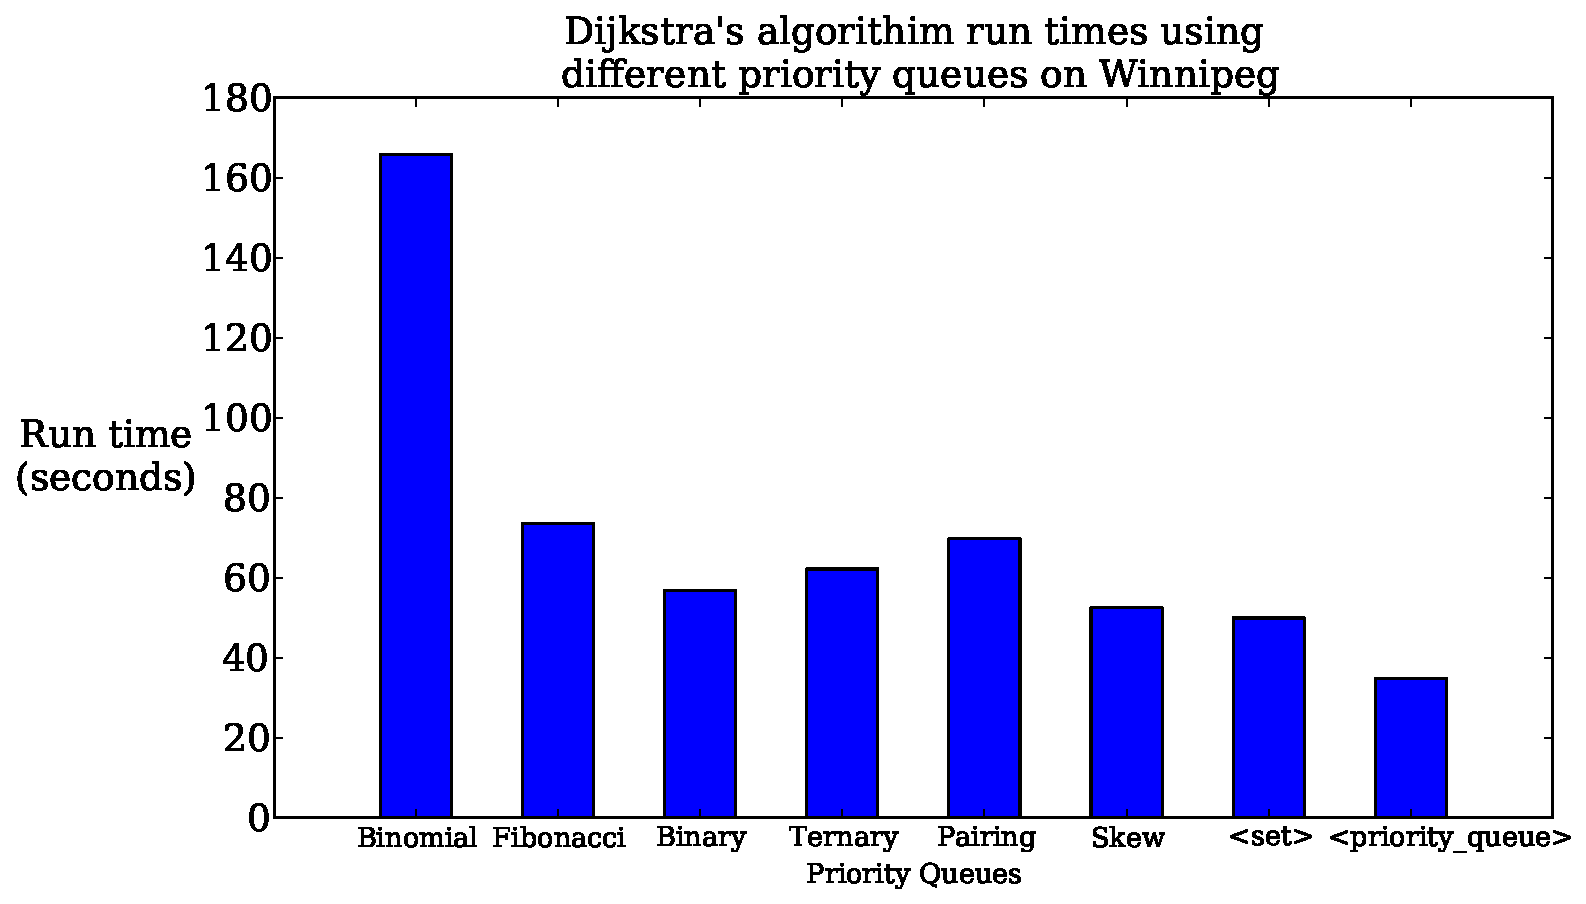
\includegraphics[width=\textwidth]{img/pq_runtime}
    \caption{Dijkstra's algorithm run times using different priority queues on ChicagoSketch}
    \label{fig:pq_runtime}
\end{figure}

Figure~\ref{fig:allresults} shows the performance of each of the algorithms
\begin{itemize}
    \item label correcting Bellman-Ford,
    %\item one source Dijkstra (1S-D),
    \item point to point Dijkstra using heap from C++ standard library,
    \item point to point Dijkstra using binary search tree,
    \item bidirectional Dijkstra,
    \item A* search,
    \item bidirectional A* search,
\end{itemize}
used on each of the networks shown in Table~\ref{table:problemdata}.
%The numbers of iterations (ITERS) each algorithm took,
\begin{figure}[H]
    \centering
    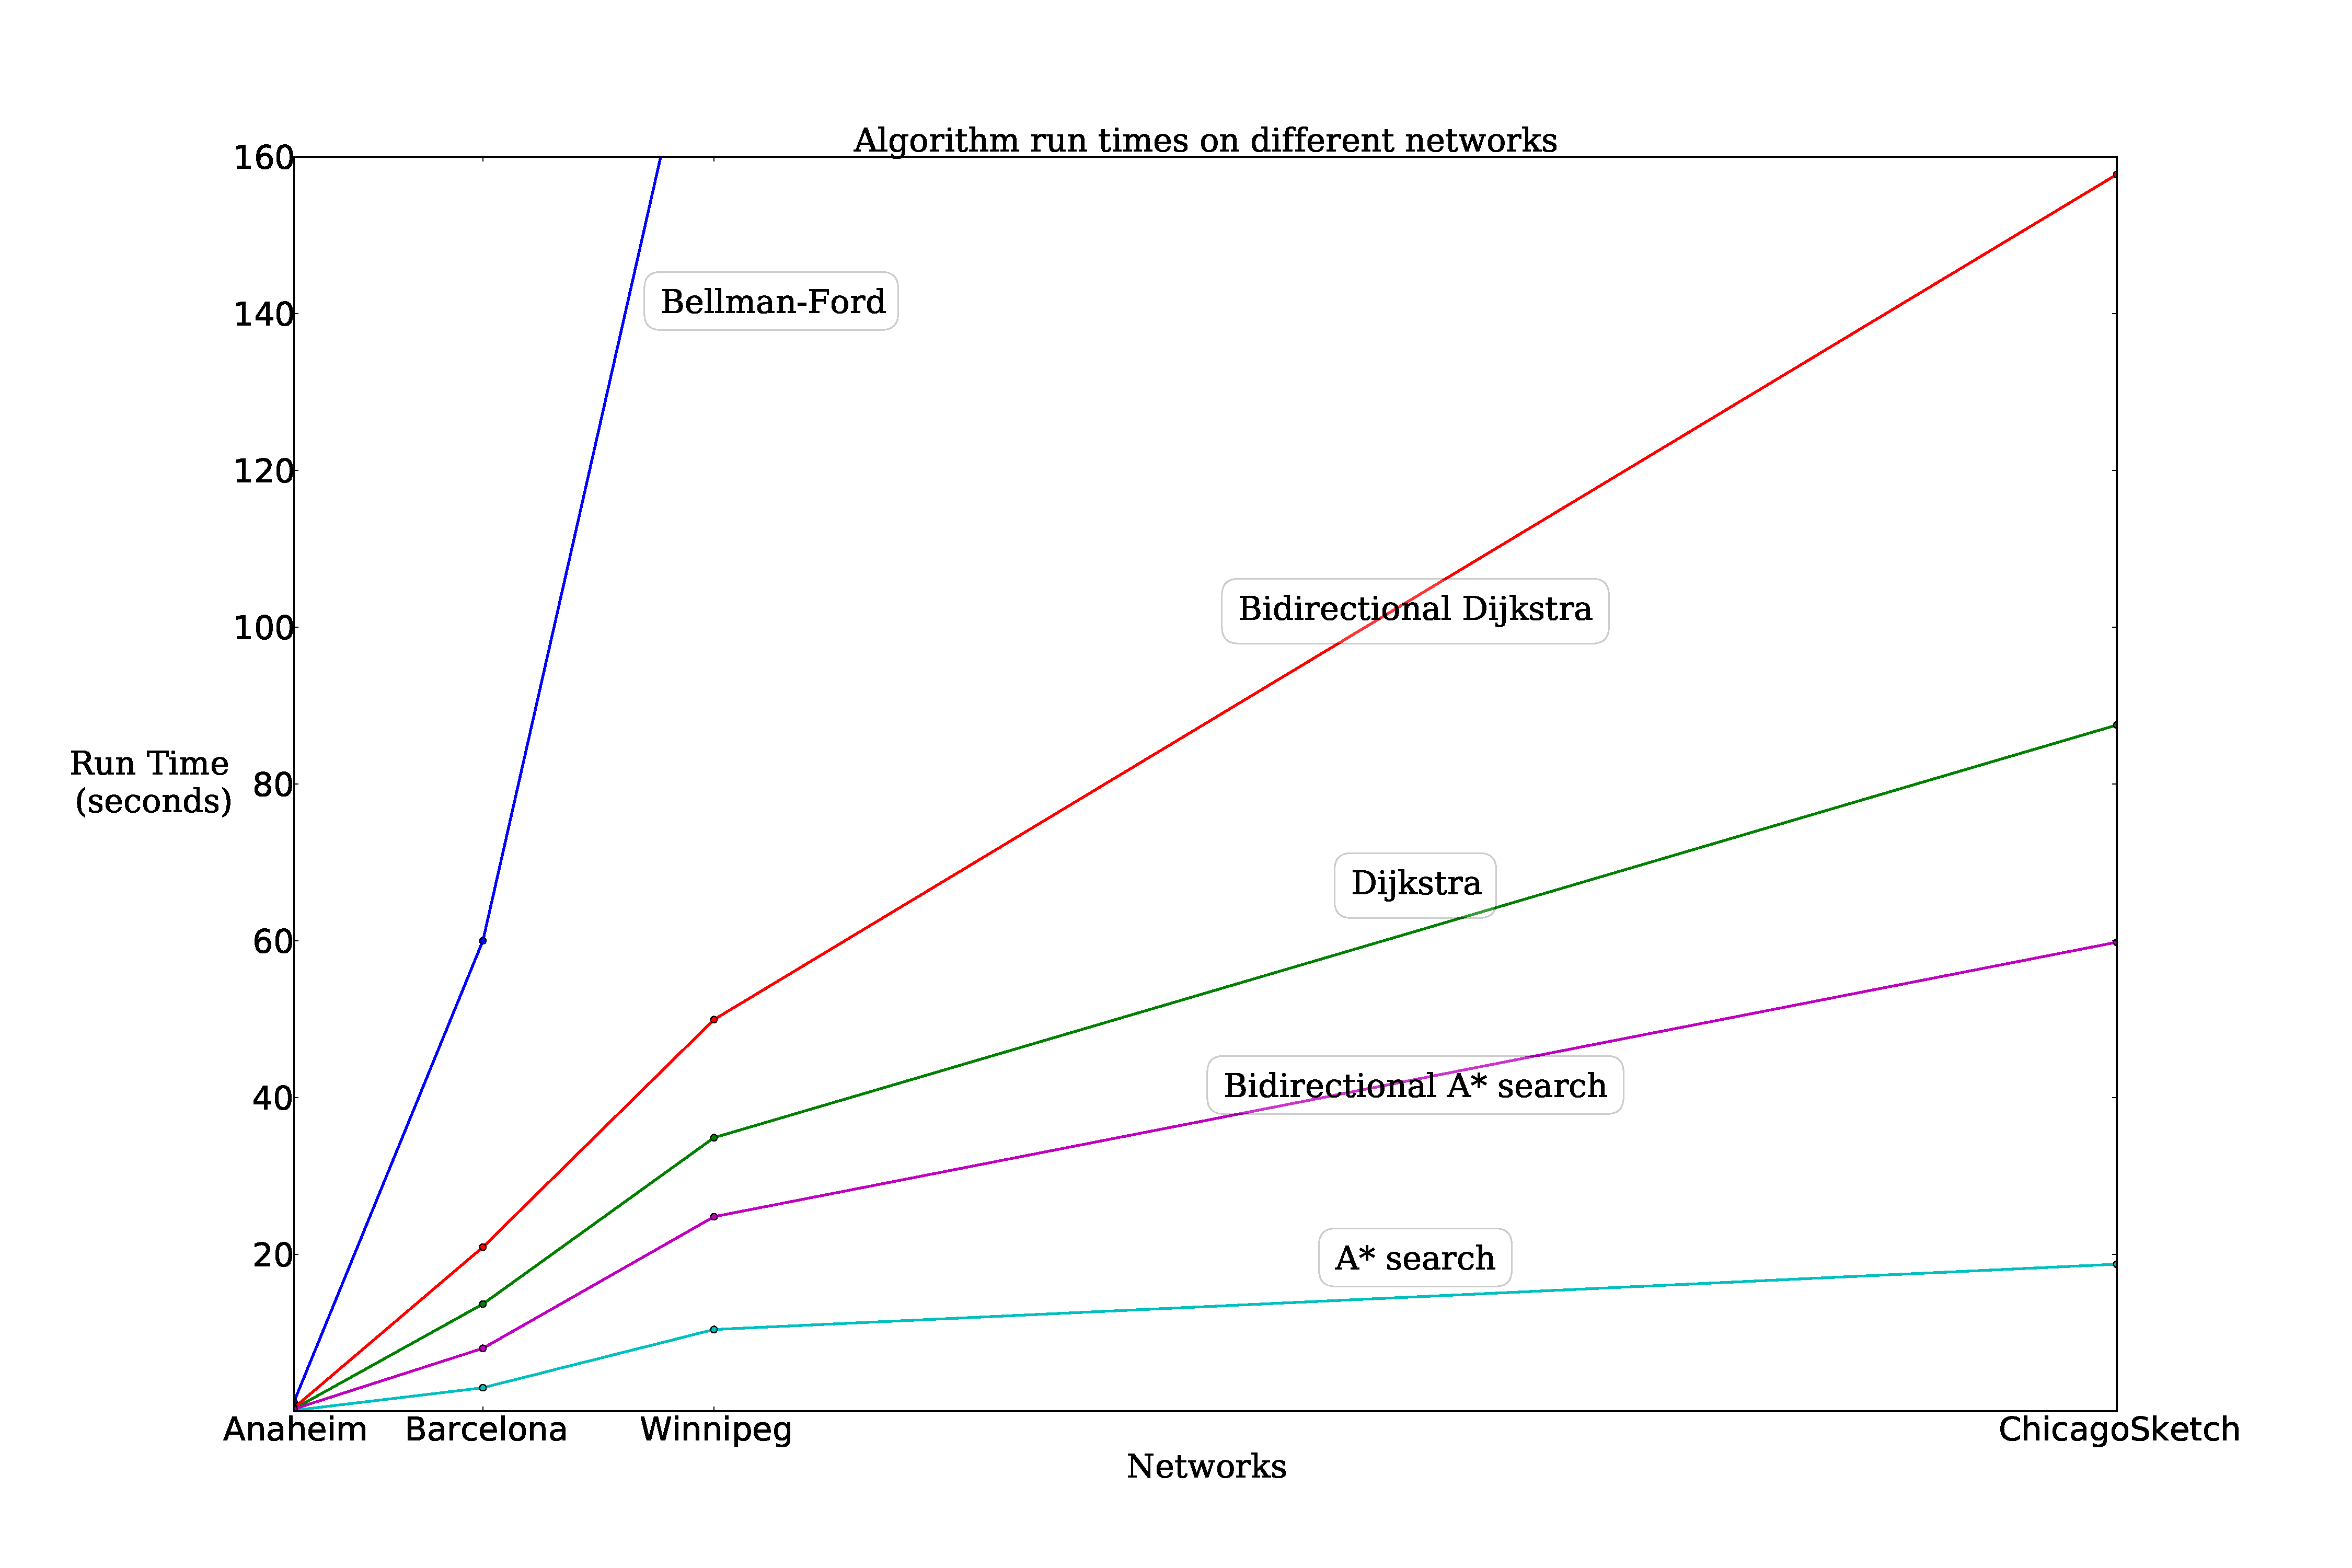
\includegraphics[width=\textwidth]{img/runtime}
    \caption{Performance of different algorithms on different networks}
    \label{fig:allresults}
\end{figure}

\begin{comment}
The overall number of nodes scanned in the network (COUNT),
and the total run time (seconds) each algorithm took is shown.
Each algorithm is also compared to the label correcting algorithm to show the percentage speed-up (SPD).
\begin{figure}[H]
    \centering
    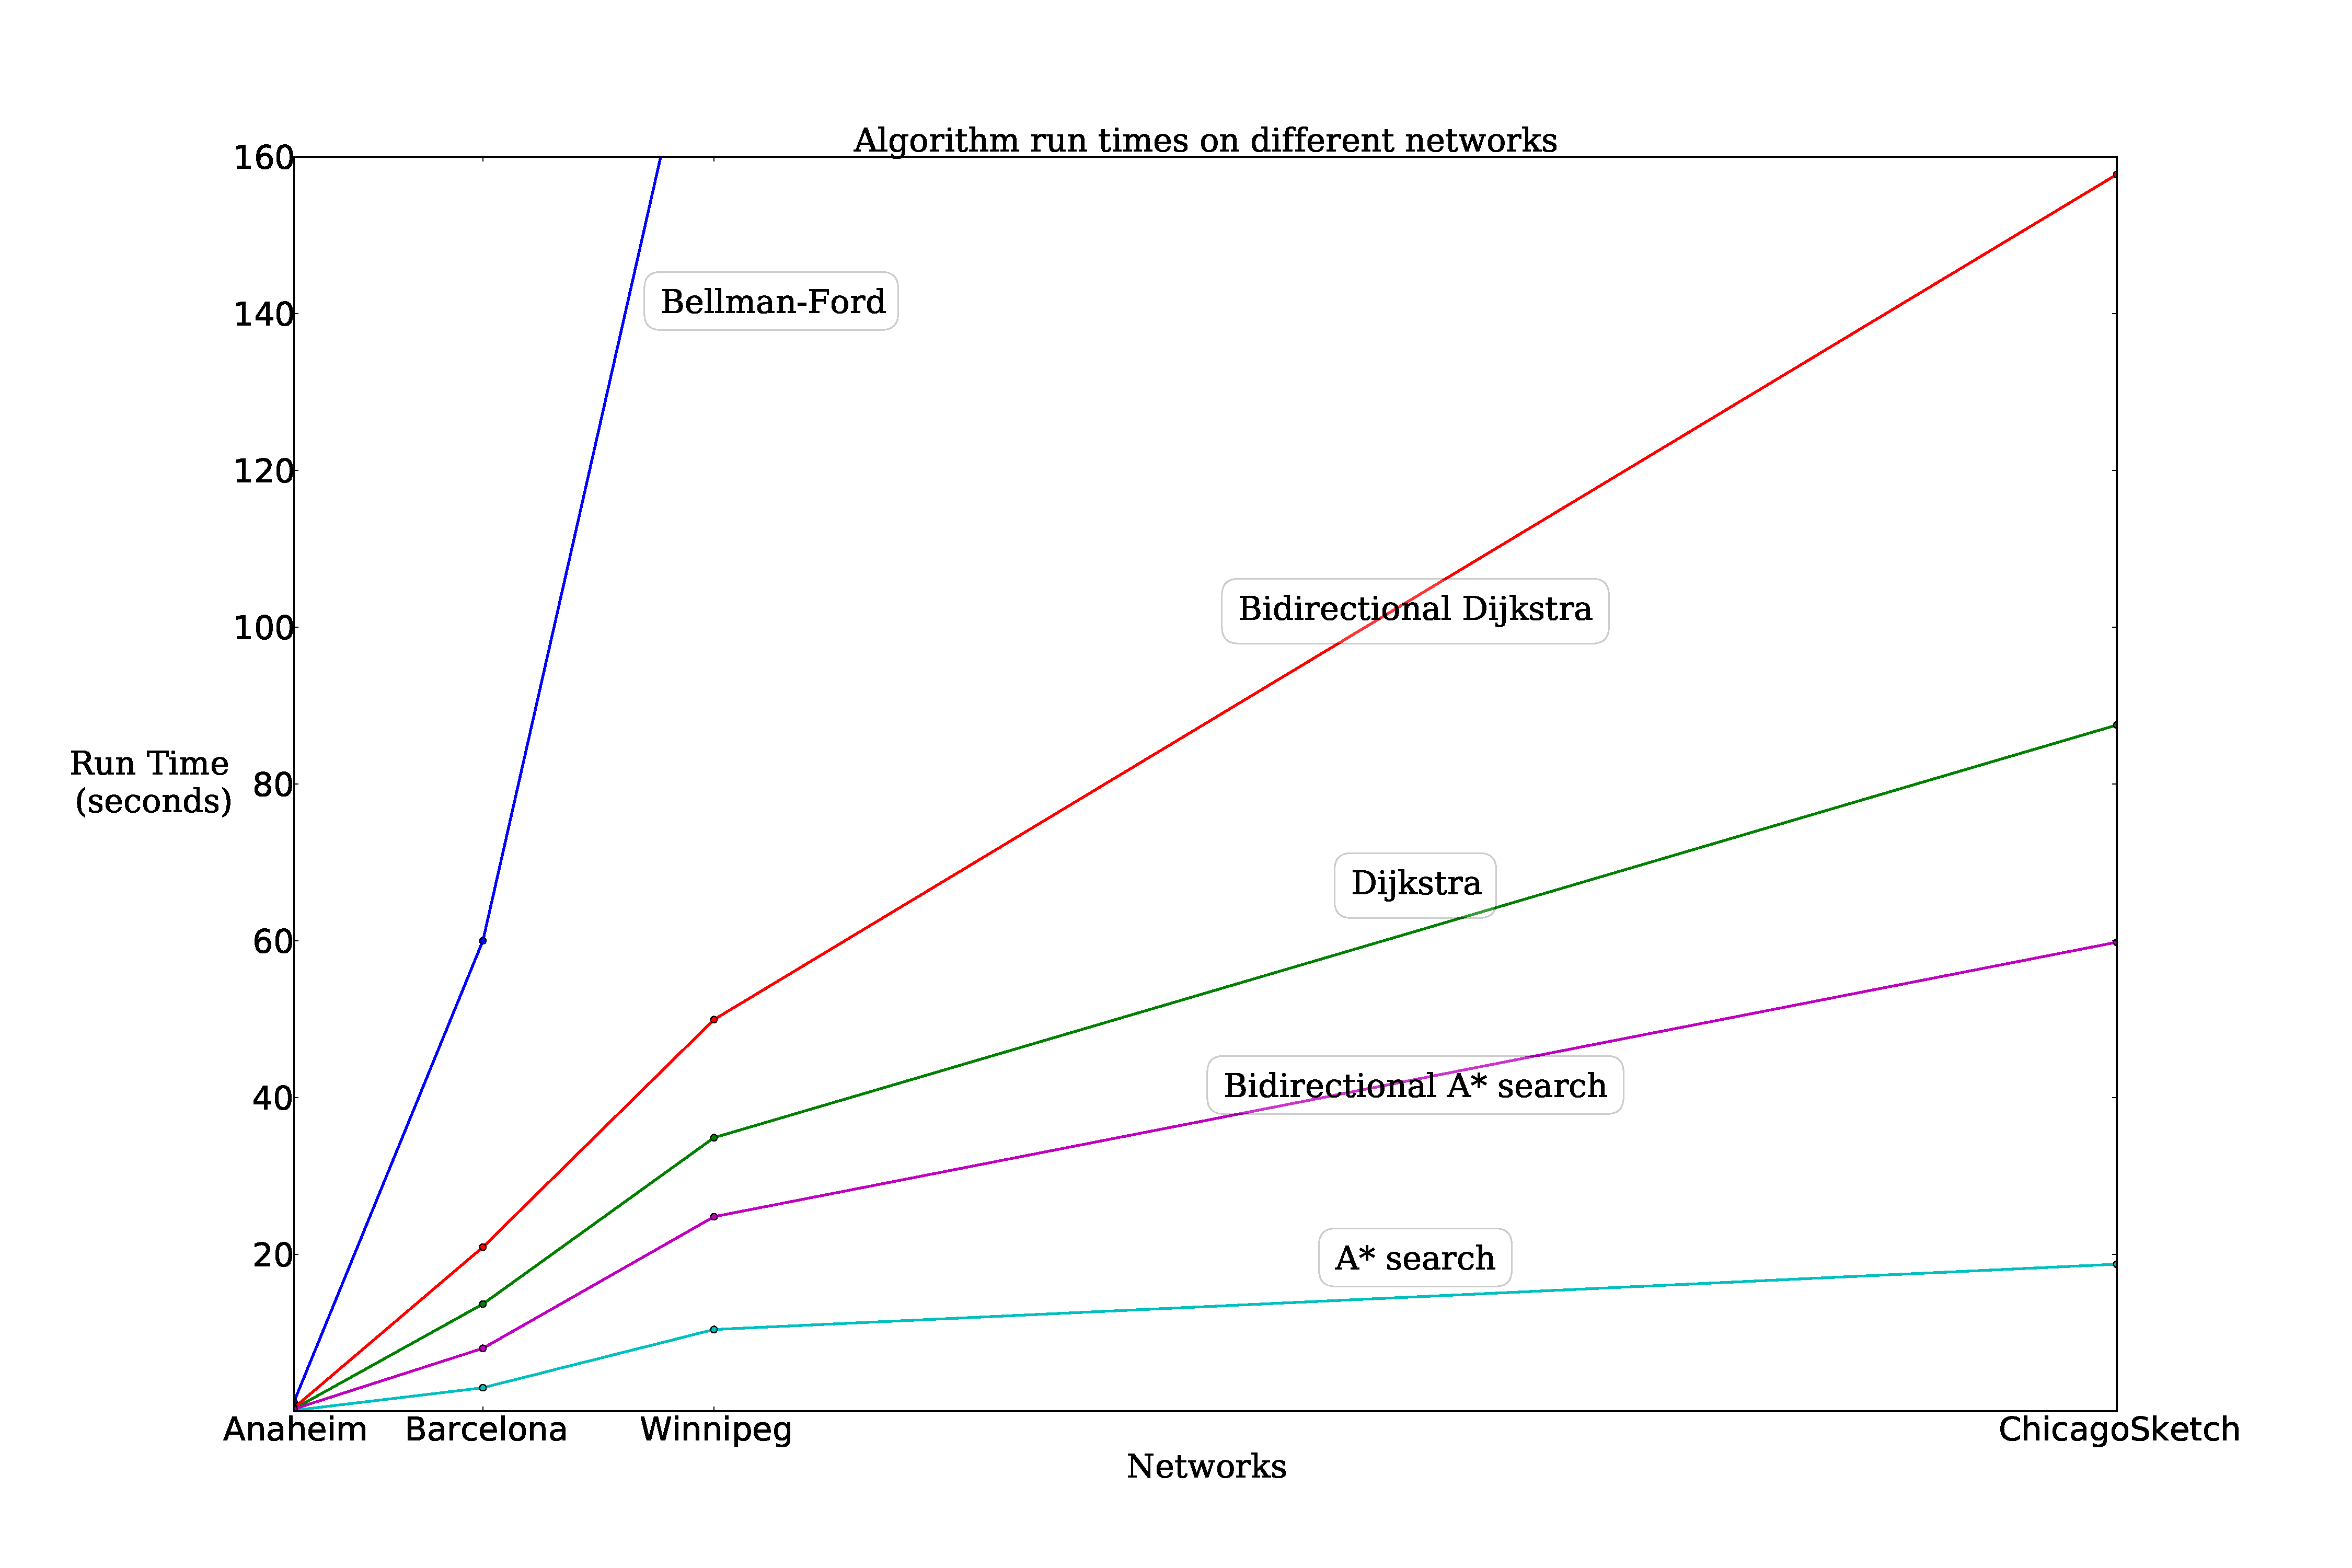
\includegraphics[width=\textwidth]{img/runtime}
    \caption{
\end{figure}

\begin{table}
    \centering
    \begin{tabular}{l l r rr rr } \toprule
        & & & \multicolumn{2}{c}{Max Scans} & \multicolumn{2}{c}{Time} \\ 
        \cmidrule(lr){4-5}
        \cmidrule(lr){6-7}
        Network & Algorithm & ITERS & COUNT & SPD                     & SEC & SPD \\ 
        \cmidrule(lr){1-1}
        \cmidrule(lr){2-2}
        \cmidrule(lr){3-3}
        \cmidrule(lr){4-4}
        \cmidrule(lr){5-5}
        \cmidrule(lr){6-6}
        \cmidrule(lr){7-7}
        SiouxFalls    & Bellman-Ford     & 69 & & & 0.25 & \\
        & Dijkstra (Heap) & 86 & & & 0.08 & \\
        & Dijkstra (Tree) & 54 & & & 0.08 & \\
        & Bidirectional Dijkstra & 87 & & & 0.16 & \\
        & A*    & 87 & & & 0.07 & \\
        & Bidirectional A* & 87 & & & 0.21 & \\ \\
        Anaheim       & Bellman-Ford    & 10 & & & 1.20 & \\
        & Dijkstra (Heap) & 10 & & & 0.30 & \\
        & Dijkstra (Tree) & 10 & & & 0.62 & \\
        & Bidirectional Dijkstra  & 10 & & & 0.43 & \\
        & A*    & 10 & & & 0.10 & \\
        & Bidirectional A* & 10 & & & 0.28 & \\ \\
        Barcelona     & Bellman-Ford    & 28 & & & 60.00 & \\
        & Dijkstra (Heap) & 27 & & & 13.67 & \\
        & Dijkstra (Tree) & 27 & & & 27.36 & \\
        & Bidirectional Dijkstra  & 27 & & & 20.93 & \\
        & A*    & 28 & & &  2.99 & \\
        & Bidirectional A* & 30 & & & 8.02 & \\ \\
        Winnipeg      & Bellman-Ford    & 129 & & & 190.00 & \\
        & Dijkstra (Heap) & 127 & & &  34.89 & \\
        & Dijkstra (Tree) & 127 & & &  66.89 & \\
        & Bidirectional Dijkstra  & 126 & & & 49.95 & \\
        & A*    & 126 & & & 10.42 & \\
        & Bidirectional A* & 127 & & & 24.81 & \\ \\
        ChicagoSketch & Bellman-Ford    & 25 & & & 500.00 & \\
        & Dijkstra (Heap) & 25 & & & 87.52 & \\
        & Dijkstra (Tree) & 25 & & & 149.95 & \\
        & Bidirectional Dijkstra  & 25 & & & 157.75 & \\
        & A*    & 26 & & & 18.75 & \\
        & Bidirectional A* & 26 & & & 59.82 & \\ \\
        \bottomrule
    \end{tabular}
    \caption{Results for all test networks. Showing the number of iterations for each network (ITERS), max number of scans (COUNT) and the speed up respect to the label correcting algorithm (SPD). }
    \label{table:allresults}
\end{table}
\todo[noline]{Result : average number of scans}
\todo[inline]{Result table for all heaps}
\end{comment}

Figure~\ref{fig:long_sptree} shows the shortest path tree between two distant nodes on the ChicagoSketch network.
We can see Dijkstra's algorithm scans the entire network.
Bidirectional Dijkstra scans almost the whole network with a few nodes not being scanned.
A* search scans only a small region of the network.
\todo{incomplete}

\begin{figure}
    \centering
    \begin{subfigure}{.5\textwidth}
        \centering
        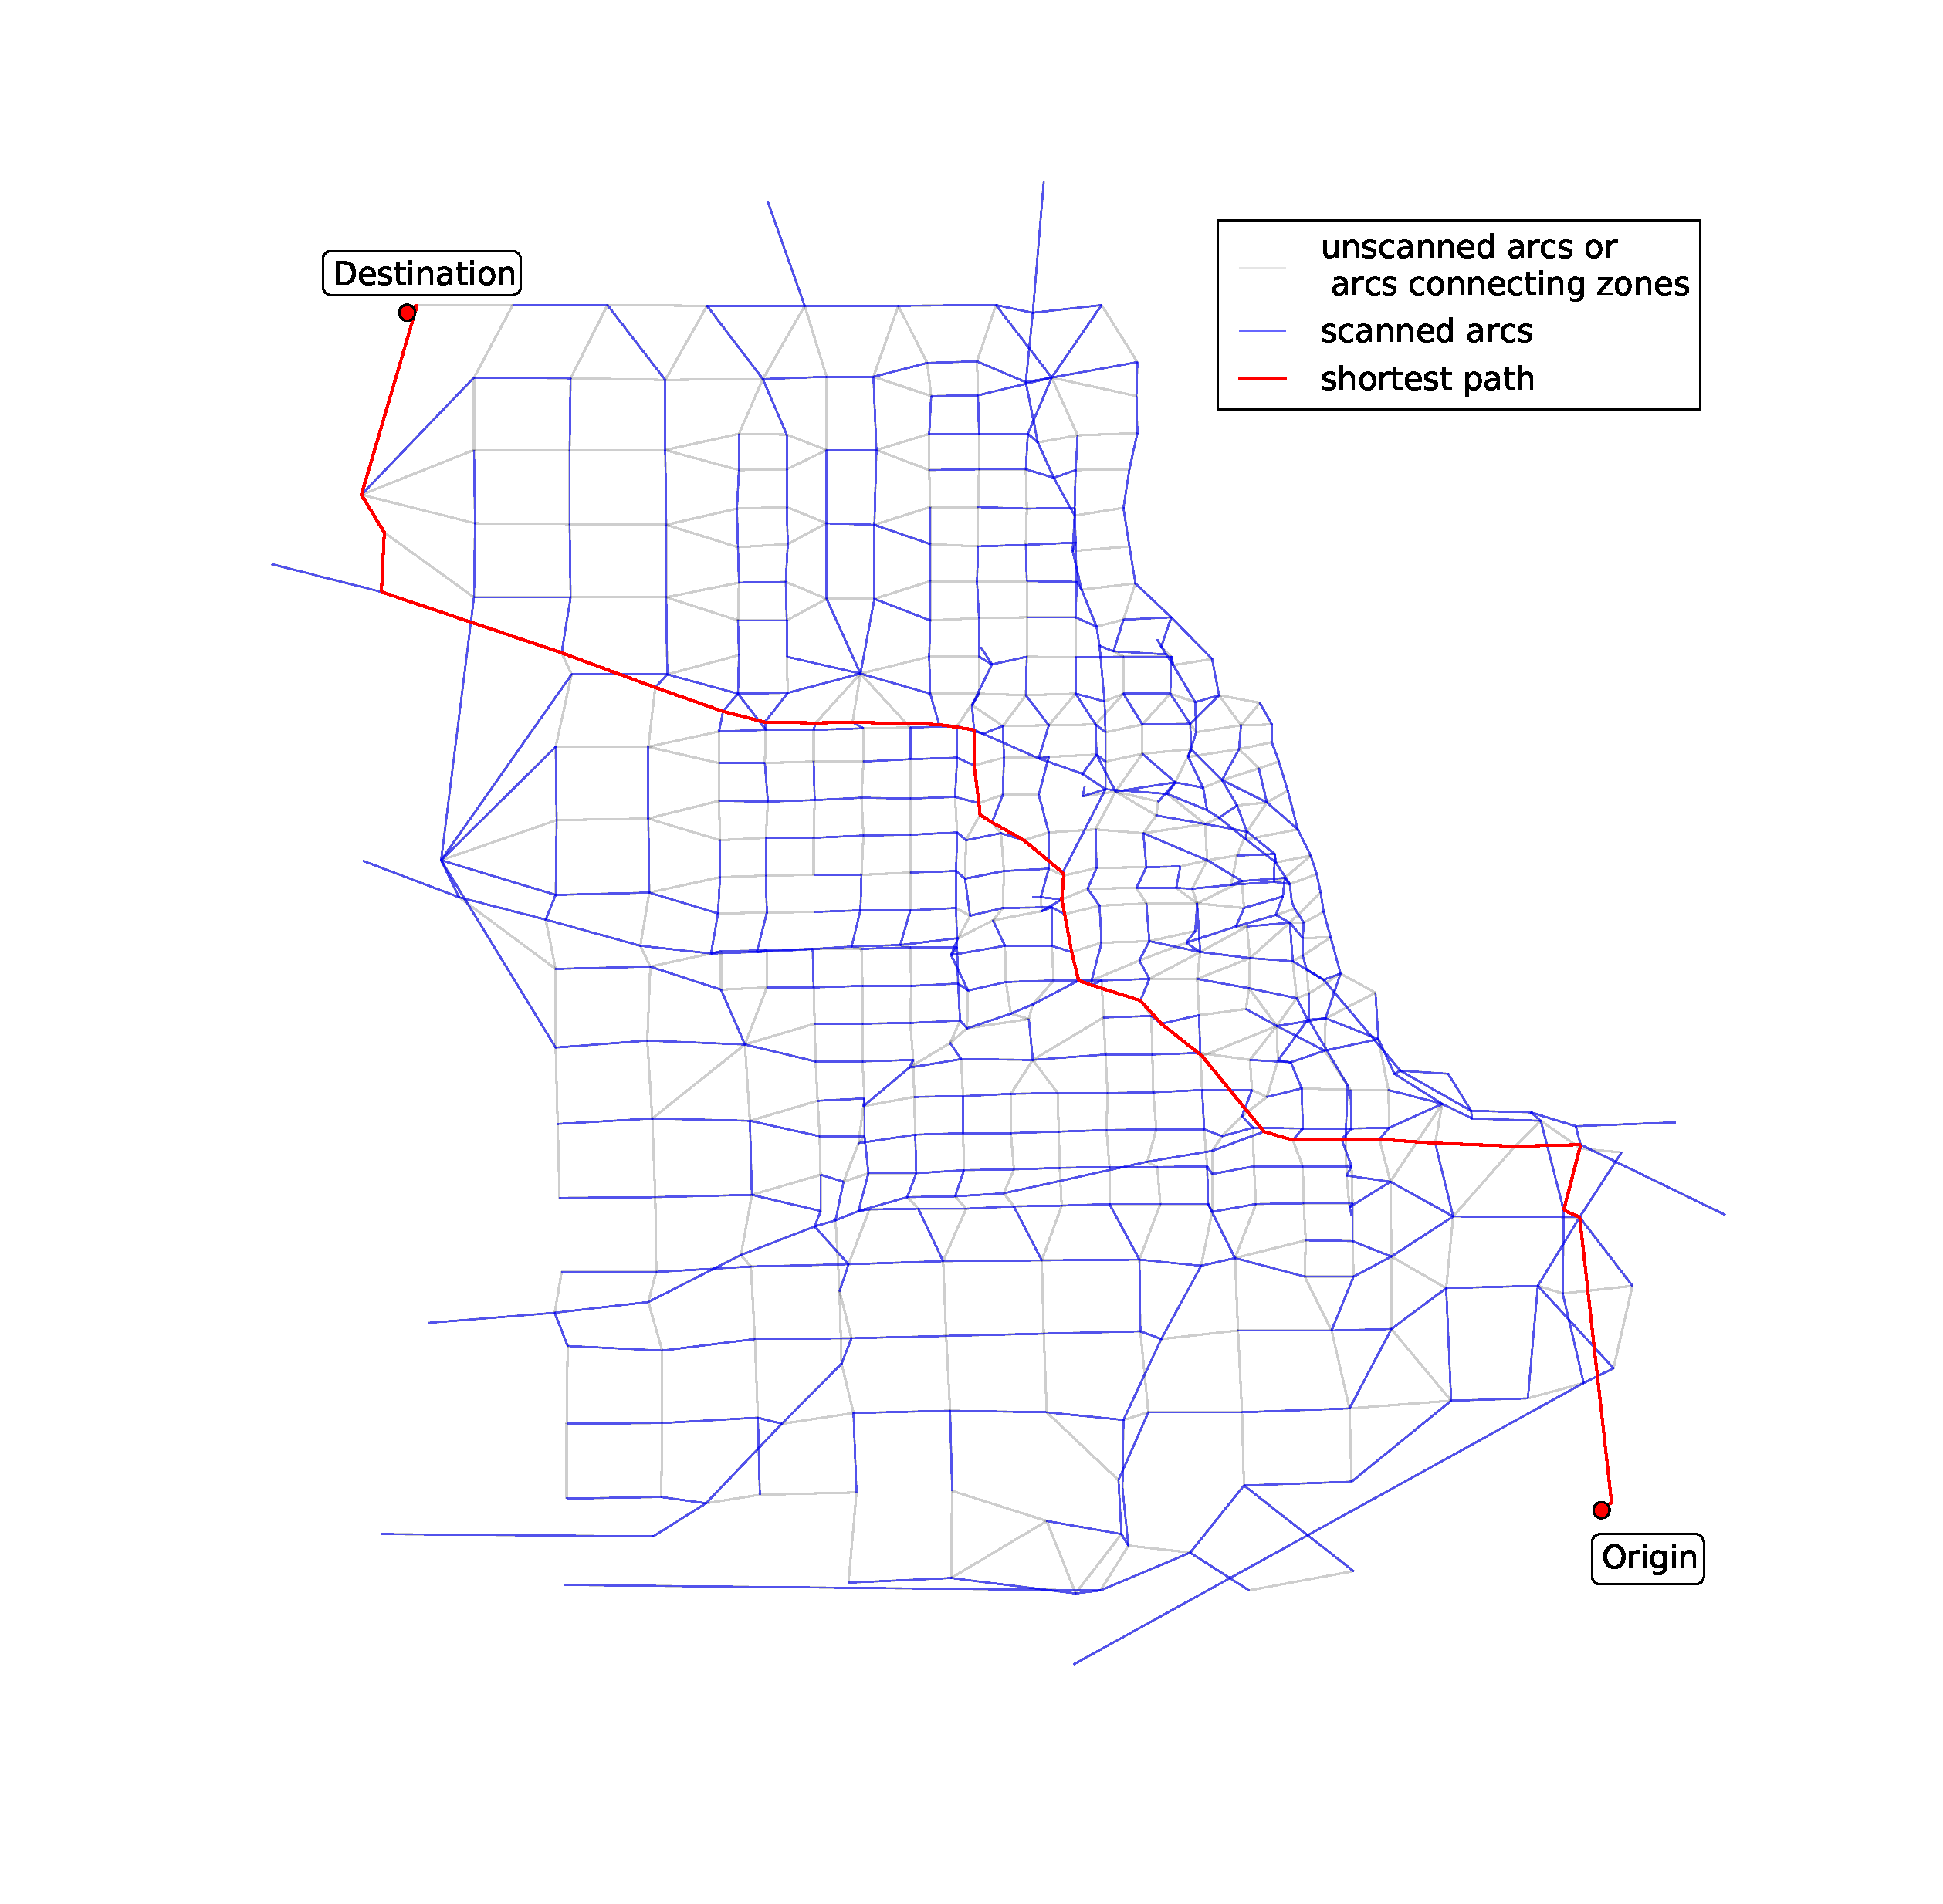
\includegraphics[width=\textwidth,trim=120px 120px 48px 120px,clip]{img/chicago_dijkstra}
        \caption{Dijkstra}
        \label{fig:chicago_dijkstra}
    \end{subfigure}%
    \begin{subfigure}{.5\textwidth}
        \centering
        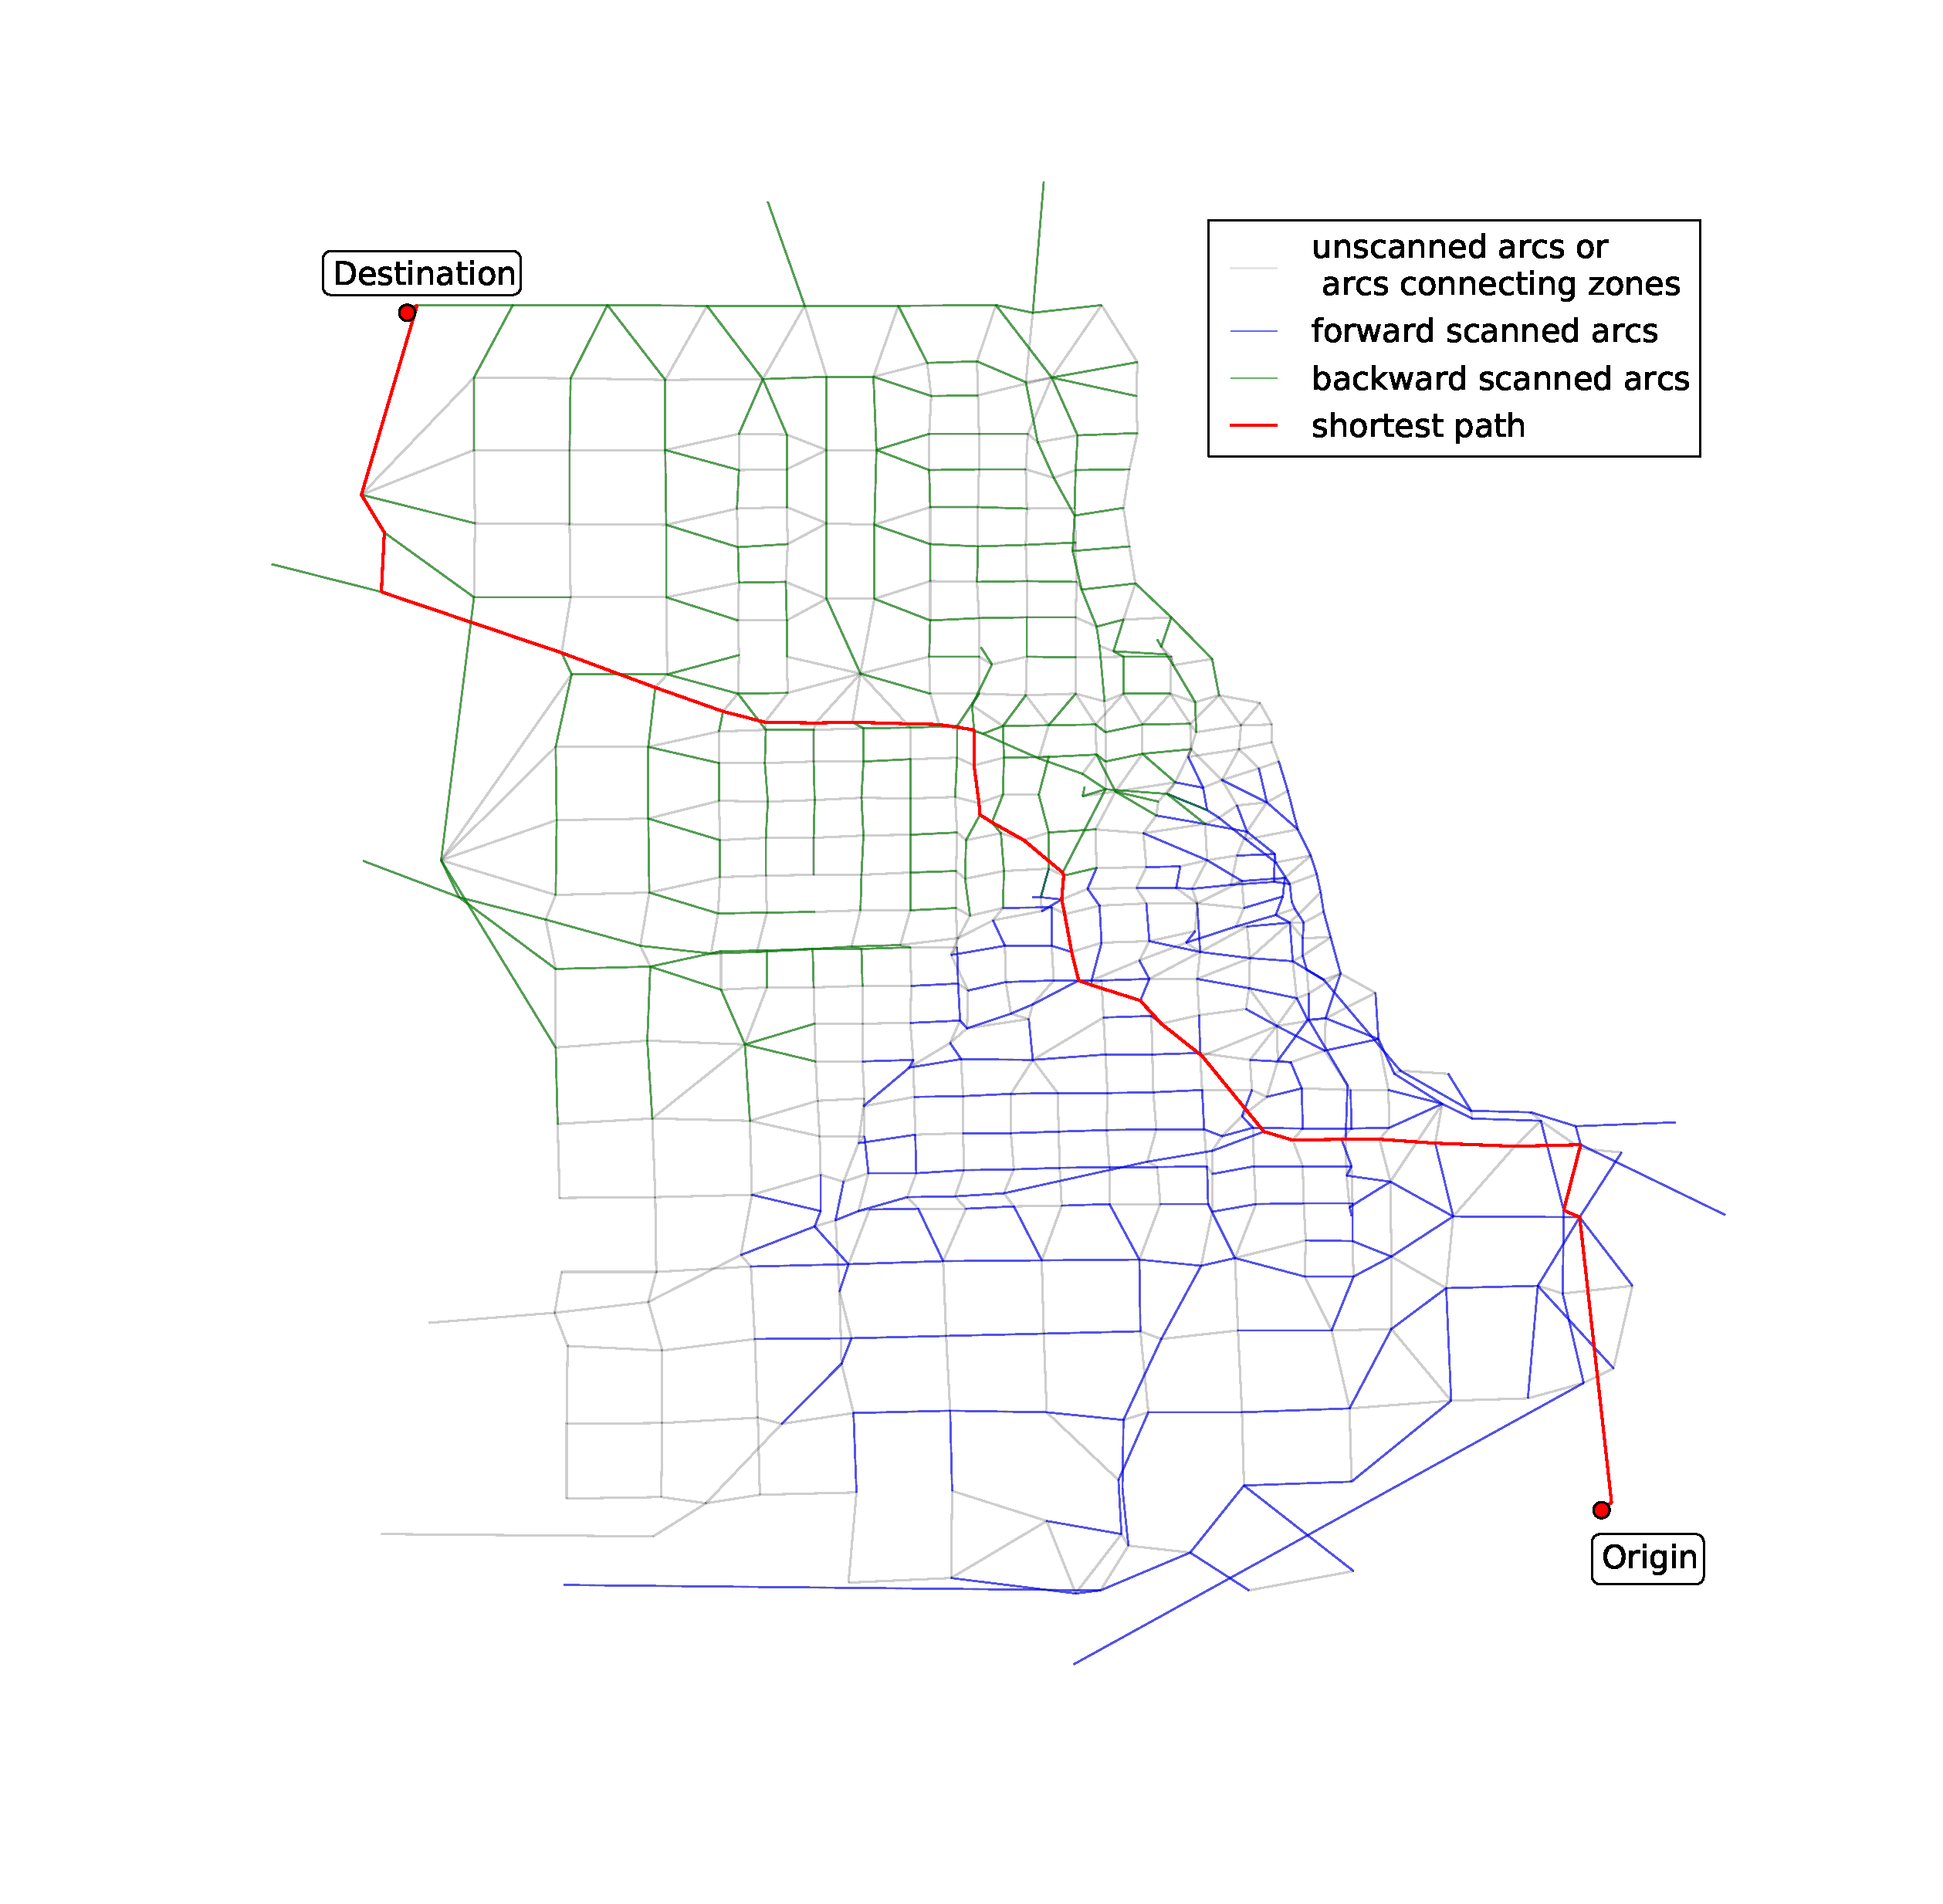
\includegraphics[width=\textwidth,trim=120px 120px 48px 120px,clip]{img/chicago_bidirect}
        \caption{Bidirectional Dijkstra}
        \label{fig:chicago_bidirect}
    \end{subfigure}
    \begin{subfigure}{.5\textwidth}
        \centering
        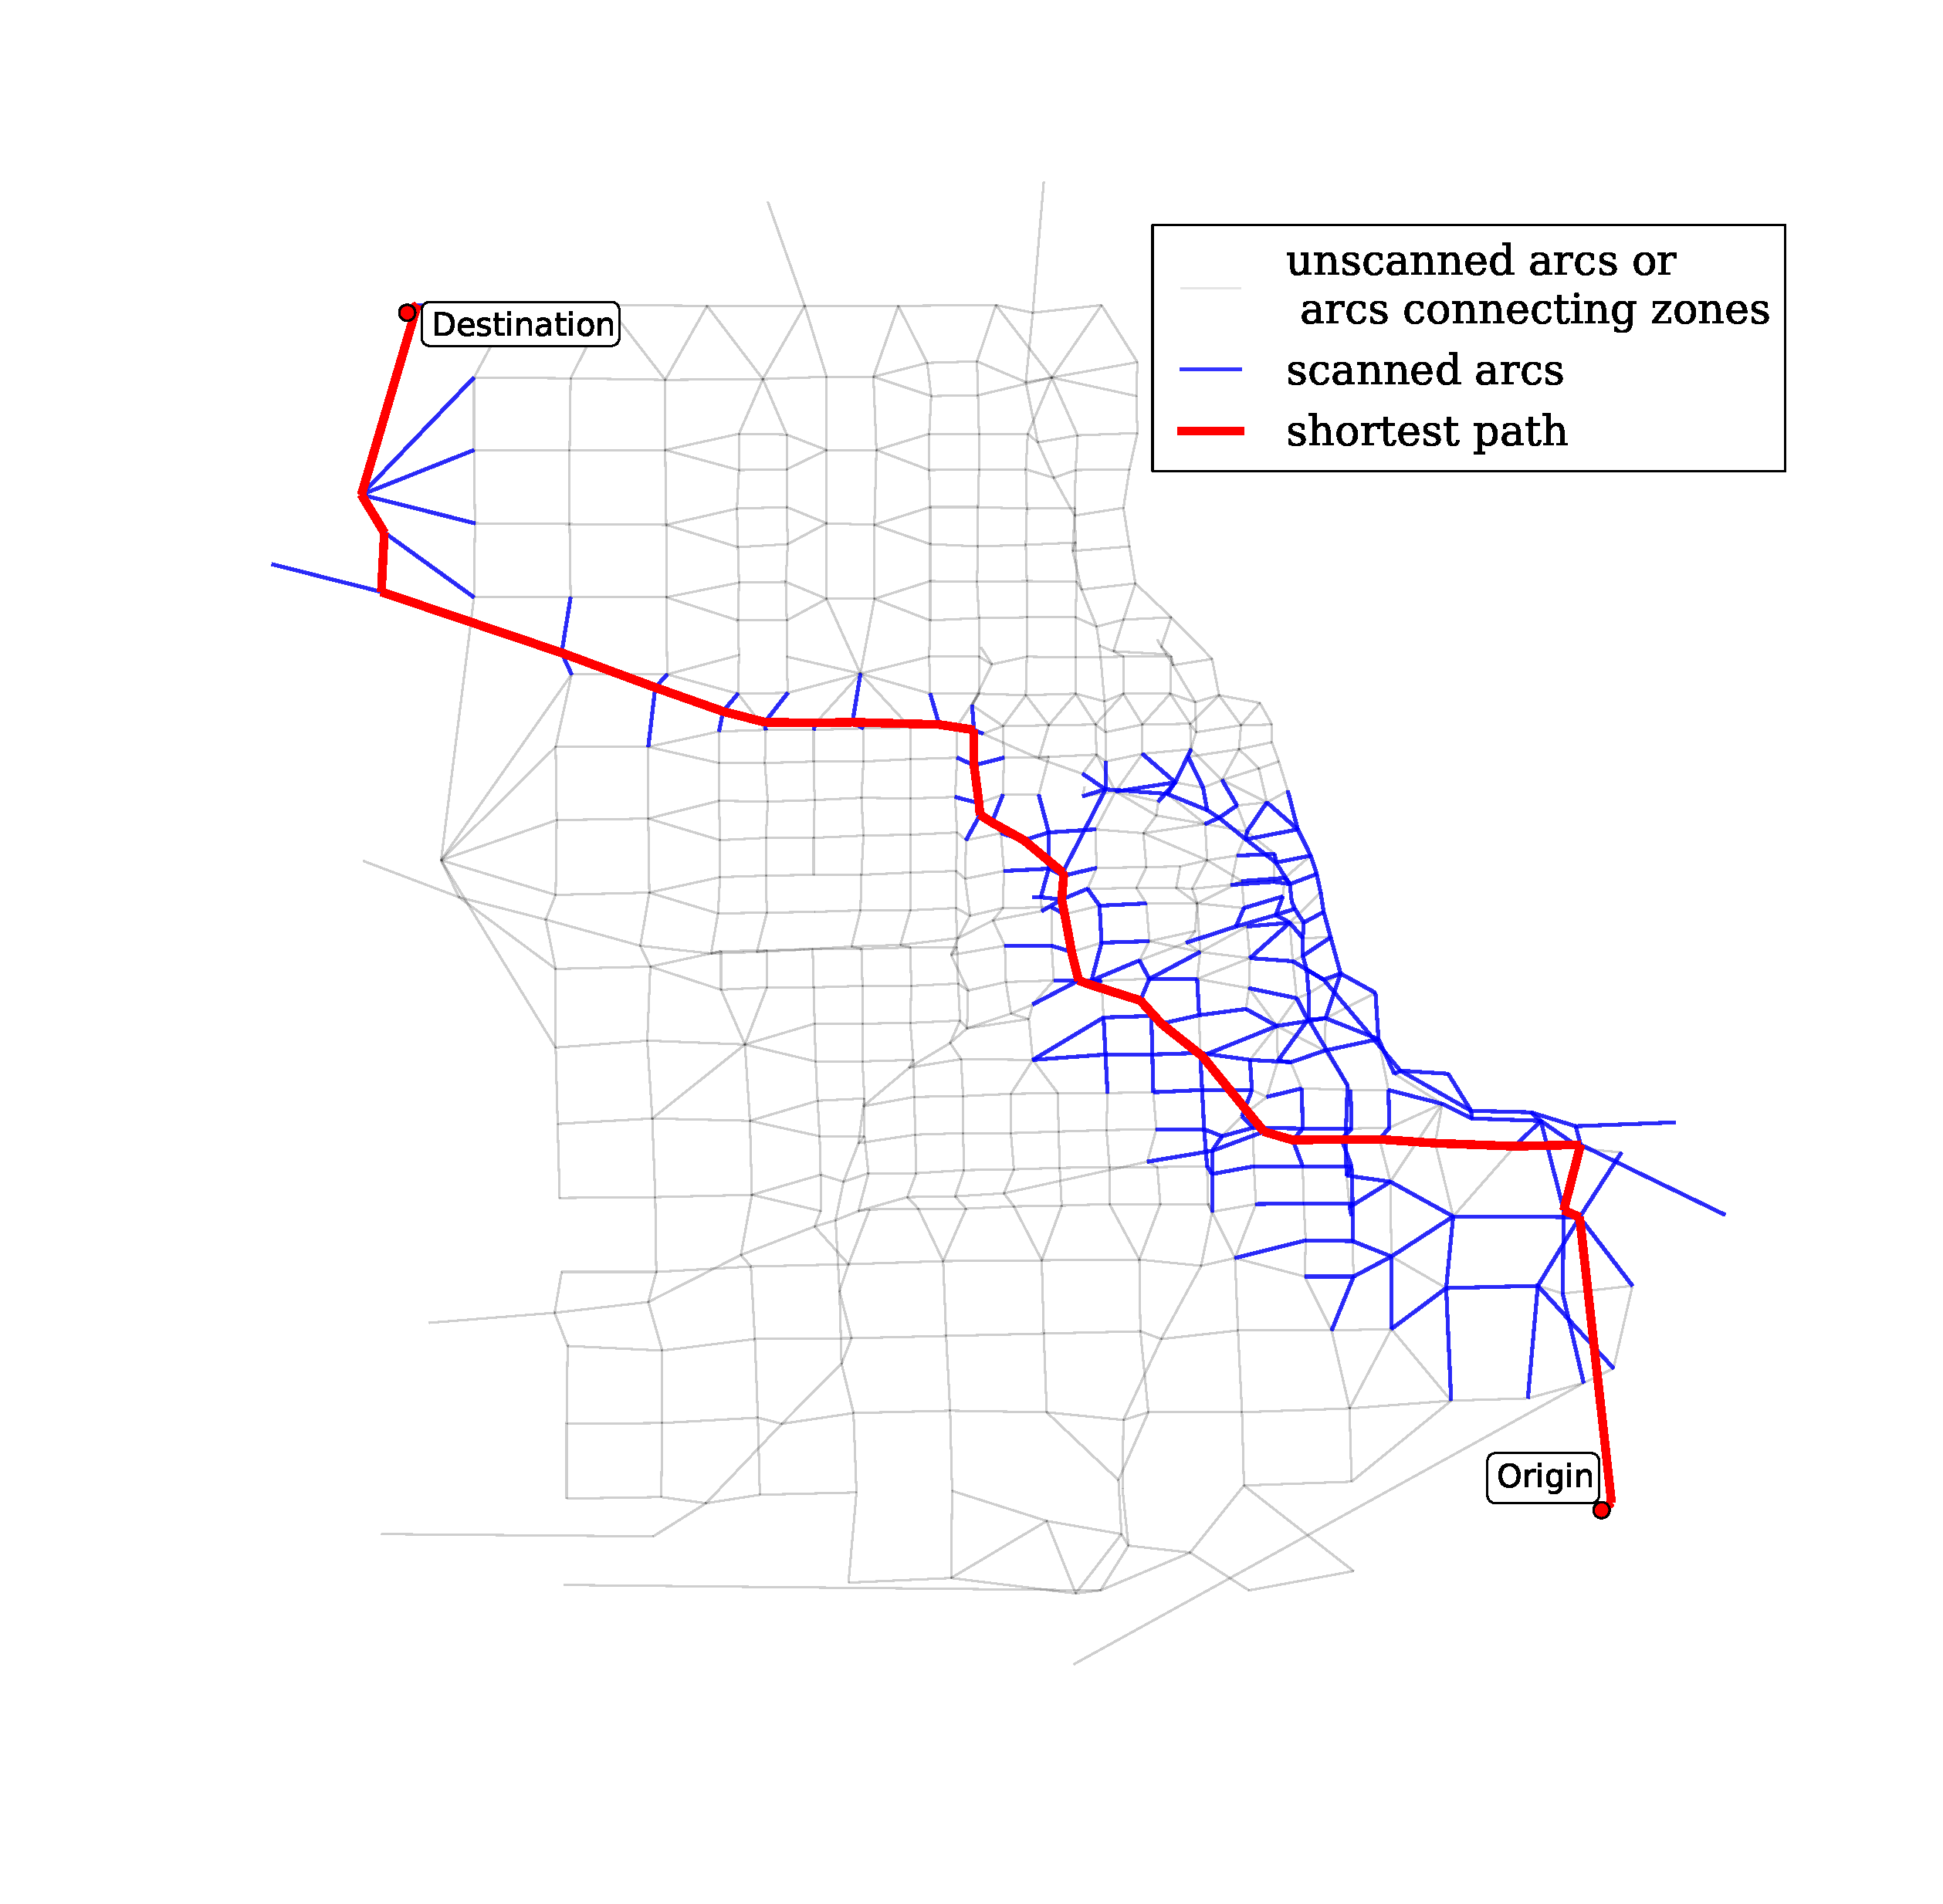
\includegraphics[width=\textwidth,trim=120px 120px 48px 0px,clip]{img/chicago_astar}
        \caption{A* Search}
        \label{fig:chicago_Astar_bidirect}
    \end{subfigure}%
    \begin{subfigure}{.5\textwidth}
        \centering
        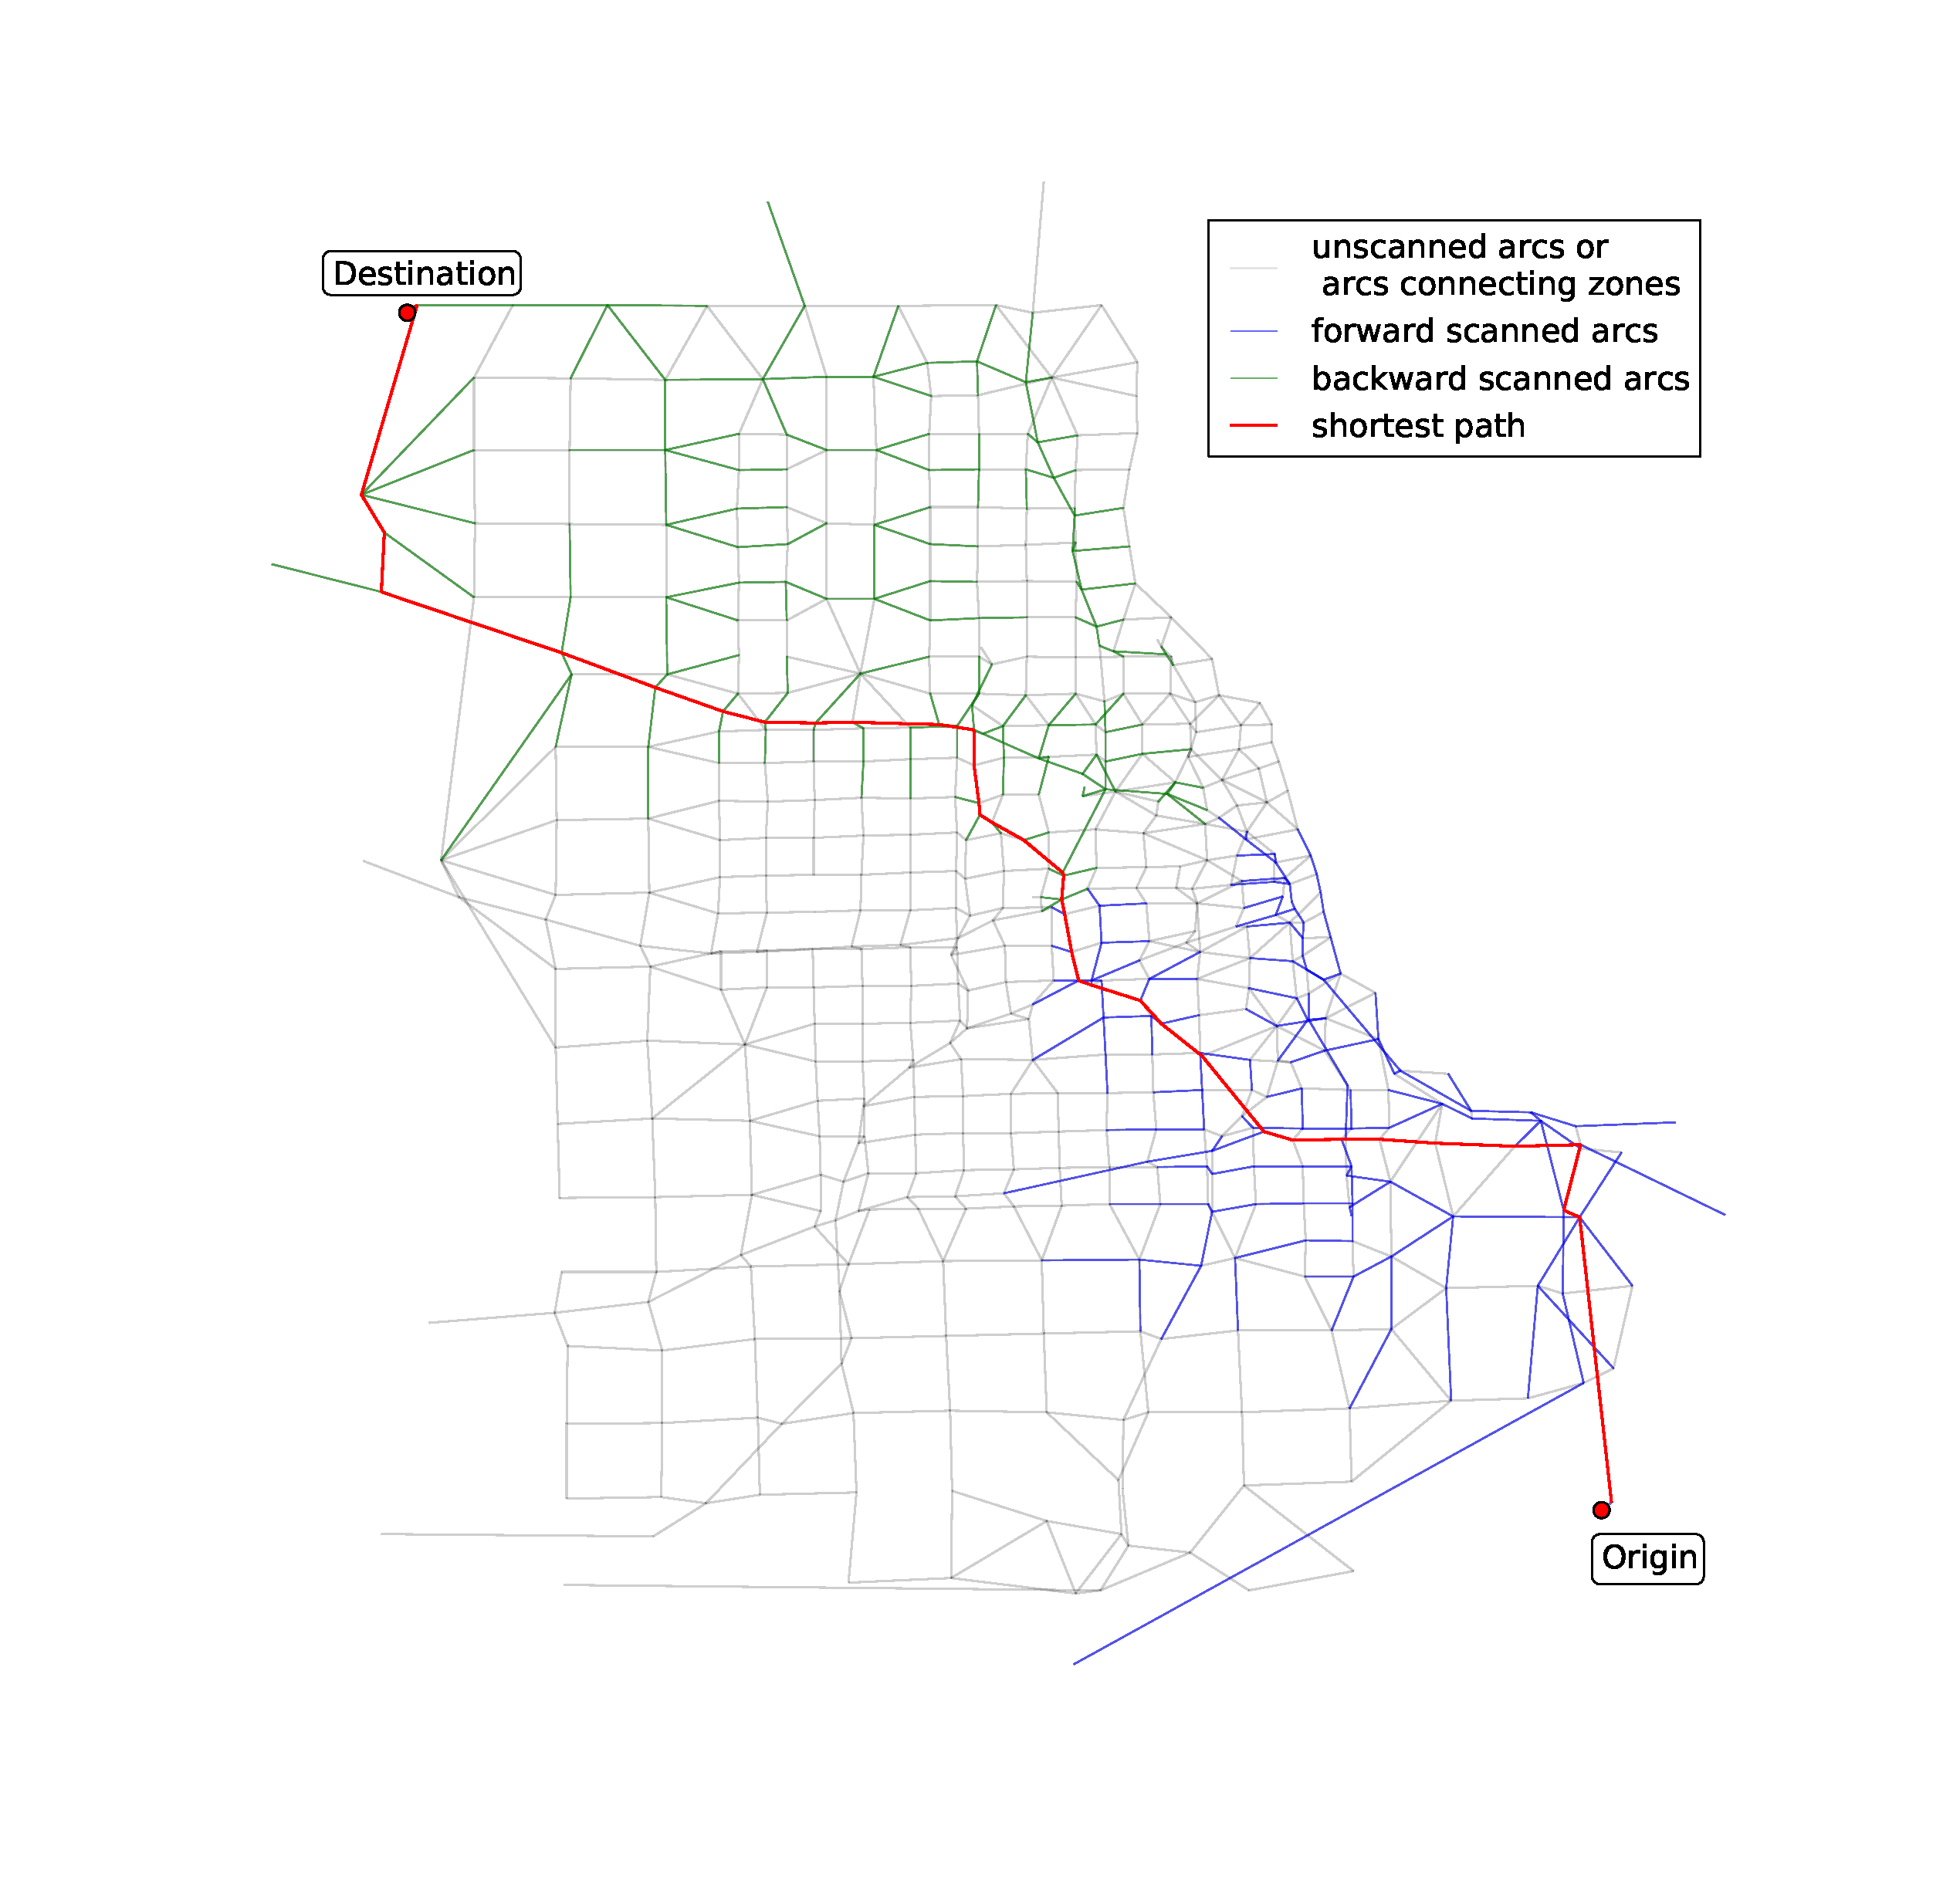
\includegraphics[width=\textwidth,trim=120px 120px 48px 0px,clip]{img/chicago_astar_bidirect}
        \caption{Bidirectional A* Search}
        \label{fig:chicago_astar_bidirect}
    \end{subfigure}
    \vspace{1em}
    \caption{Shortest Path Tree between Two Distant Nodes in the ChicagoSketch Network -D Pair}
    \label{fig:long_sptree}
\end{figure}
\todoin{draw 2 nodes that are close to each other}


\begin{comment}

All of these run times are slower than the STL version of the Heap.
Upon inspection,
it is found that the increase-key operation is used about between 5\% to 10\%
of the time,
\todo{not actual count yet}
which means the graphs are not dense enough for these Heap structures to outperform a
simple array based priority queue.
Comparing the Dijkstra and A* search algorithm's result,
we see an approximately 5 times improvement.
By looking at the shortest path tree generated
by the ChicagoSketch network,
there are only a few scanned nodes,
the path goes straight to the destination.
(TODO reference) says the closer the heuristic is to the actual distance,
the better/faster shortest path calculation,
by looking at the travel time function (Figure~\ref{fig:flowfunction}, we can see the slope
is really shallow near the start,
and by comparing the initial flow and final flow (TODO, data),
they are very close so the final flow is very close to the
initial flow,
which means the heuristic is a very good estimation,
which is our A* search is very fast.
\end{comment}
\todo[inline]{give results interpretation}

\begin{figure}[H]
    \centering
    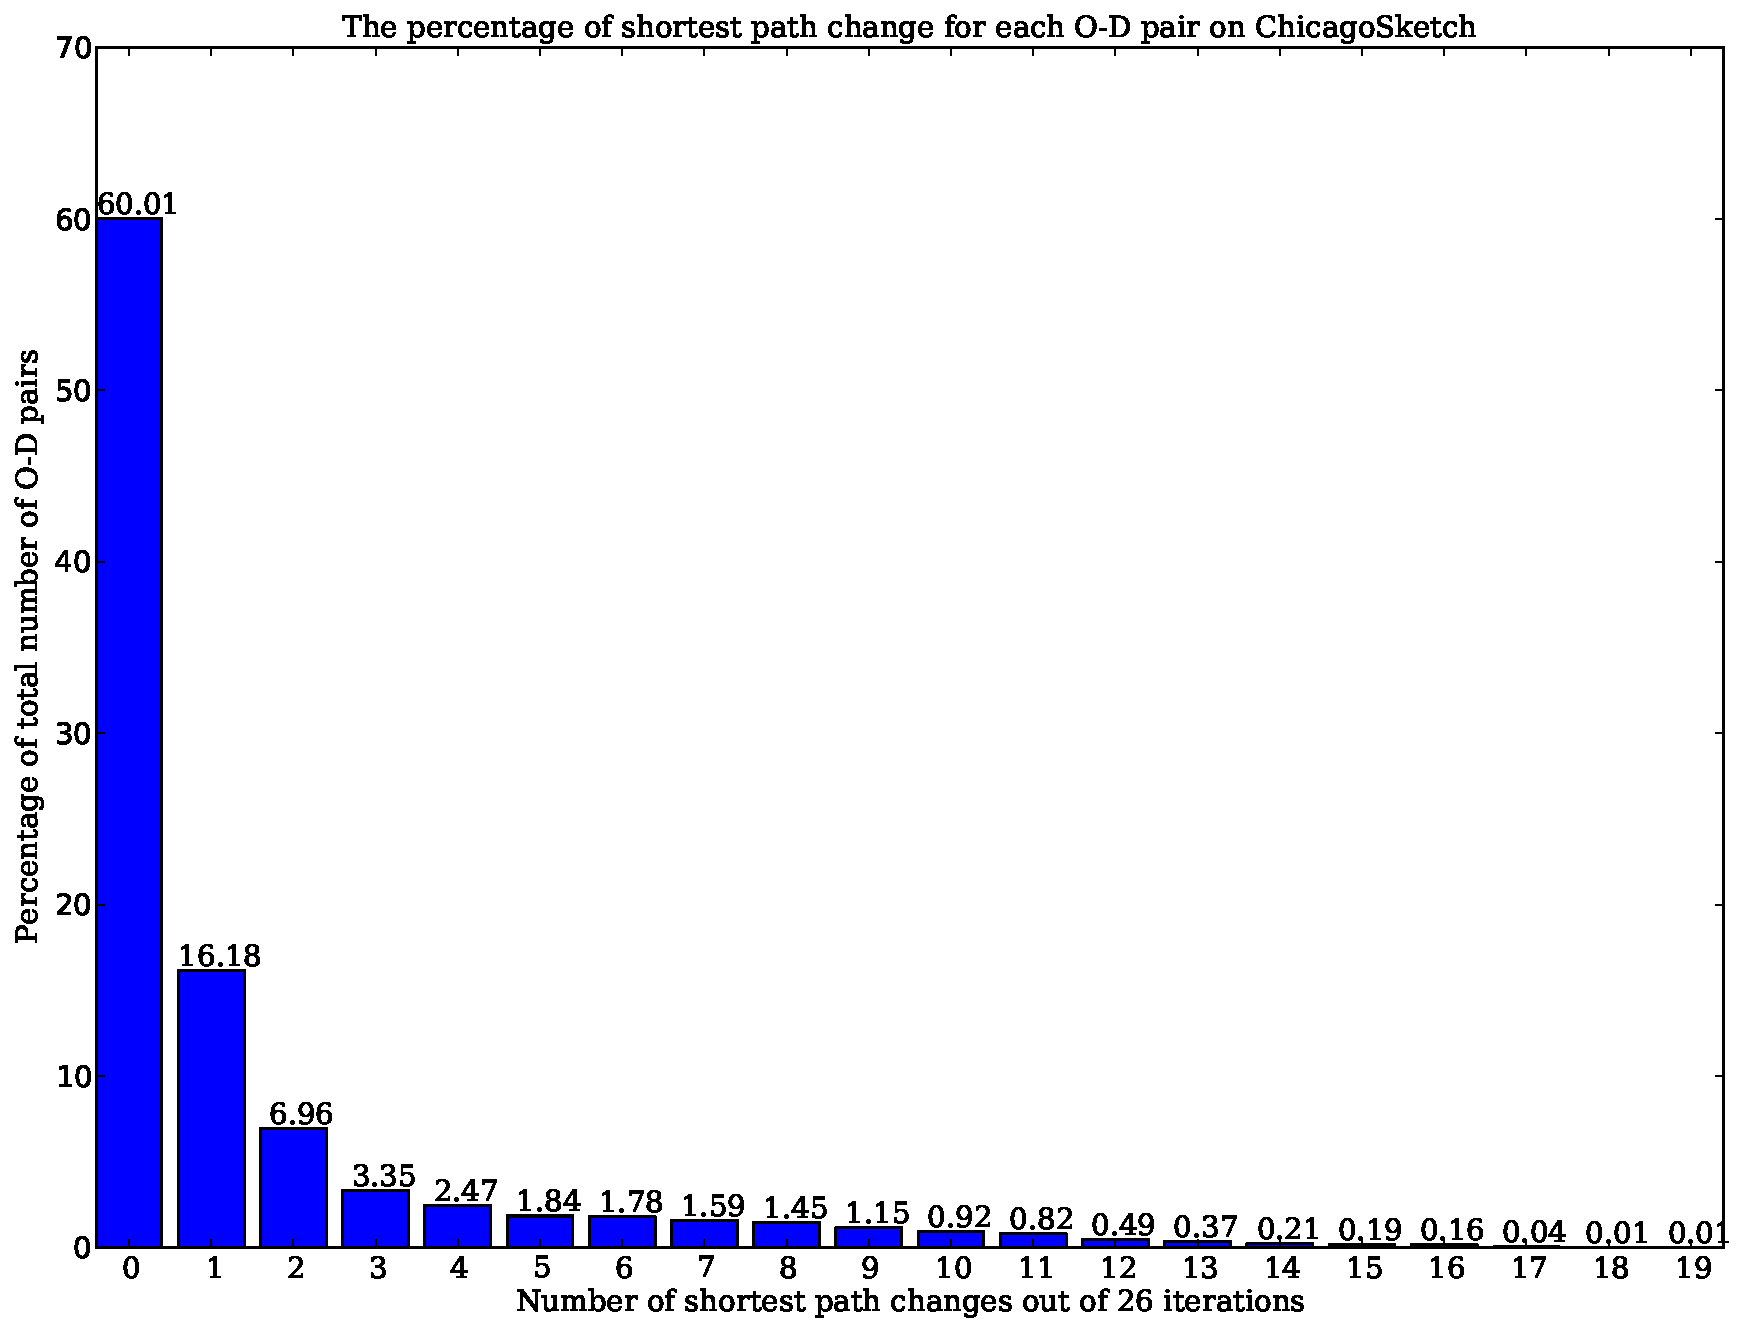
\includegraphics[width=\textwidth]{img/sp_change}
    \caption{The percentage of shortest path change for each O-D pair out of 26 iterations for ChicagoSketch}
    \label{fig:sp_change}
\end{figure}


